% GENERATED by latex/convert.py from 'Autonima - Manuscript.docx'.
% Edit the Google Doc and re-run, or adopt this file and stop running it.
\section{Abstract}

Systematic meta-analysis enables cumulative science, but expert-led workflows do not scale with the growing literature. In neuroimaging, automated synthesis frameworks are widely used but are less precise than expert synthesis due to coarse article selection and pooling of all reported analyses, even when only a subset is relevant. Here we present AutoNIMA, a large language model (LLM)-guided framework that automates article screening according to expert-defined eligibility criteria and parses heterogeneous tables to extract coordinates and select individual analyses for quantitative meta-analysis. Against a benchmark of nine published meta-analyses, AutoNIMA recovered published maps more closely than keyword-based baselines in 26 of 28 target contrasts, frequently while pooling fewer analyses. Critically, the improvement arose not from better article selection but from identifying the analyses relevant to each question. These findings establish analysis-level selection as key to more precise neuroimaging meta-analysis and demonstrate how structured LLM guidance can scale expert-defined evidence synthesis.

\section{Introduction}

The rapid expansion of the scientific literature makes scalable synthesis essential for researchers to integrate findings and stay abreast of new evidence\cite{Bornmann2021-qk}. In neuroimaging, quantitative meta-analysis assesses spatial convergence in brain activity or structural differences across studies\cite{Eickhoff2009-hf}, helping researchers evaluate evidence beyond individual experiments. Despite the availability of integrated curation platforms\cite{Kent2026-qb,Laird2005-qq}, systematic efforts remain laborious. Estimates indicate biomedical syntheses require over a thousand research hours\cite{Allen1999-pw} and over a year on average to complete\cite{Borah2017-nf}. As a result, automated methods have become widely used, supporting exploratory meta-analysis, large-scale cognitive mapping and the interpretation of experimental findings \cite{Yarkoni2011-hi,Dockes2020-ka,Poldrack2012-qk,De_la_Vega2016-qb,Rubin2017-nh}.

Although automated meta-analytic methods have advanced from term-based text mining to predictive modelling and learned representations \cite{Dockes2020-ka,Hammonds2026-yb,Ghayem2026-vx,Peraza2025-mi,Ngo2022-if}, two technical barriers limit their precision. First, semantic relevance does not establish eligibility, which requires carefully interpreting participants, tasks and experimental designs against explicit researcher-defined criteria\cite{Muller2018-zo}. Second, neuroimaging articles report brain coordinates in tables containing multiple analyses with heterogeneous layouts, making automated extraction difficult. As a result, existing automated frameworks aggregate all analyses reported in the same article. This pooling combines distinct tasks, participant groups or opposing contrasts and can include ineligible analyses, such as region-of-interest (ROI) analyses in whole-brain meta-analysis. More recently, there have been successful efforts that apply large language models (LLMs) to screen biomedical studies against researcher-defined criteria\cite{Cao2025-pt,Issaiy2024-gp,Chen2026-fl}, resulting in expert-level systematic literature reviews, suggesting the potential to apply contextual automated screening to specific neuroimaging results, enabling more precise automated meta-analyses.

Here we present AutoNIMA, an LLM-guided framework that applies expert-defined eligibility criteria to neuroimaging articles and the individual analyses within them. AutoNIMA implements an end-to-end workflow encompassing literature search, article screening, coordinate extraction, analysis-level selection and coordinate-based meta-analysis. Using NeuroMetaBench, a companion benchmark comprising nine published expert-conducted meta-analyses and 32 target contrasts, we assess agreement with expert curation and compare recovery of published maps against keyword-based baselines. We isolate the contributions of article screening and analysis selection to determine which decisions improve spatial fidelity. By making this workflow broadly available, AutoNIMA enables rapid, targeted neuroimaging synthesis as a routine part of research.

\section{Results}

\subsubsection{Overview of AutoNIMA and its evaluation}

AutoNIMA uses expert-defined eligibility criteria to configure a sequential screening pipeline that yields a meta-analytic map for each target contrast (Fig.~\ref{fig:workflow}). The workflow searches PubMed, screens abstracts and then evaluates available full texts against more detailed article-level criteria. For eligible articles, heuristics locate candidate coordinate tables, and LLMs separate their coordinates into individual analyses. Each analysis is then evaluated against contrast-specific criteria using the surrounding article context. This distinction between article and analysis eligibility is central: a relevant article may report several experimental comparisons, only some of which address a particular target. Coordinates from selected analyses are submitted to coordinate-based meta-analysis to produce the final maps.

\begin{figure}[htbp]
\centering
\fbox{\begin{minipage}[c][7cm][c]{0.96\linewidth}\centering
\textsf{\large [ Figure 1 -- schematic in preparation ]}
\end{minipage}}
\caption{\textbf{AutoNIMA workflow from research question to meta-analytic map.} a, Researchers specify article-level eligibility criteria and contrast-specific criteria for individual analyses. b, PubMed search retrieves candidate article records and abstracts. c, An LLM screens abstracts, then available full texts, returning eligibility decisions with supporting rationales and criterion-level assessments; articles proceed when all inclusion criteria are met and no exclusion criteria apply. d, Heuristics identify candidate coordinate tables, which LLMs parse into distinct analyses and coordinates. e, Each analysis is assessed against contrast-specific criteria in the context of its article and assigned to eligible targets. f, Selected coordinates enter coordinate-based meta-analysis to generate a map for each target contrast.}
\label{fig:workflow}
\end{figure}

We evaluated our framework using NeuroMetaBench, a companion benchmark comprising nine published expert-conducted meta-analyses and 32 target contrasts. We assessed agreement at each curation stage and compared map correspondence with expert references against keyword-based.

\textbf{Expert-defined criteria improve screening precision while retaining relevant studies}

We manually defined criteria for each of the nine reference meta-analyses, initially following the criteria reported by the original authors as closely as possible. Manual review identified and corrected major omissions in two projects. Further LLM-assisted refinement using benchmark feedback yielded modest additional gains in map correspondence (Fig.~\ref{fig:tiers}). We report screening results using the best-performing configuration for each project.

Article screening progressively improved precision of included studies relative to the manual benchmark (Fig.~\ref{fig:screening}b). Precision, measured as the proportion of retained articles appearing in the benchmark inclusion list, increased monotonically at every stage in all nine projects, improving from an average of 10.3\% after PubMed search to 32.3\% after full text screening, and 47\% when retaining only articles with at least one analysis selected for a target contrast. However, qualitative inspection identified several plausibly relevant articles among the apparent false positives, suggesting that differences between the literature retrieved by the original reviewers and our PubMed searches could lower measured precision. To assess this possibility, we repeated screening using candidate article lists obtained from the original authors---available for only three of the nine projects---while holding eligibility criteria constant. Across these three projects, mean final precision increased from 49.7\% to 65.7\%, a difference of 16 percentage points ( Fig.~\ref{fig:pools}), indicating closer agreement between LLM-guided screening and expert curation when candidate study pools were aligned.

To distinguish screening performance from data availability, we evaluated recall relative to the benchmark studies available for assessment at each stage. Studies lacking usable article text or coordinate data were excluded from the denominator, while screening-based exclusions remained counted as errors. Mean recall remained at 81.8\% after analysis-level selection, with an 18.2-percentage-point decrease compared with a 36.7-percentage-point increase in precision.

\begin{figure}[htbp]
\centering
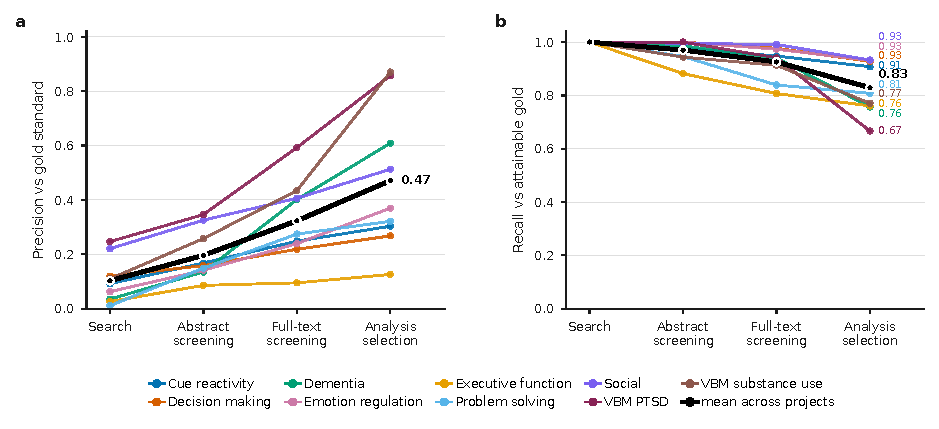
\includegraphics[width=\linewidth]{../../reports/nature_methods_figures/figure2_precision_and_attainable_recall.pdf}
\caption{\textbf{Screening improves precision while retaining most available expert-included articles.} \textbf{a}, Precision of included studies, relatively to the benchmark, increases monotonically across stages of the pipeline. \textbf{b}, Availability-adjusted recall across the same stages decreases moderately across pipeline stages, with an average of 82\% of candidate benchmark studies retained in the final stage. Articles not retrieved by the search, no available full text or yielding no coordinate tables in the main text are excluded from the denominator at the corresponding stage. Search-stage recall is therefore 100\% by construction and does not indicate complete retrieval of the benchmark literature. In both panels, colored lines represent individual projects (\emph{n} = 9), and the mean metrics are represented in black.}
\label{fig:screening}
\end{figure}

\textbf{Automated coordinate parsing and analysis-level selection\\
}\begin{figure}[htbp]
\centering
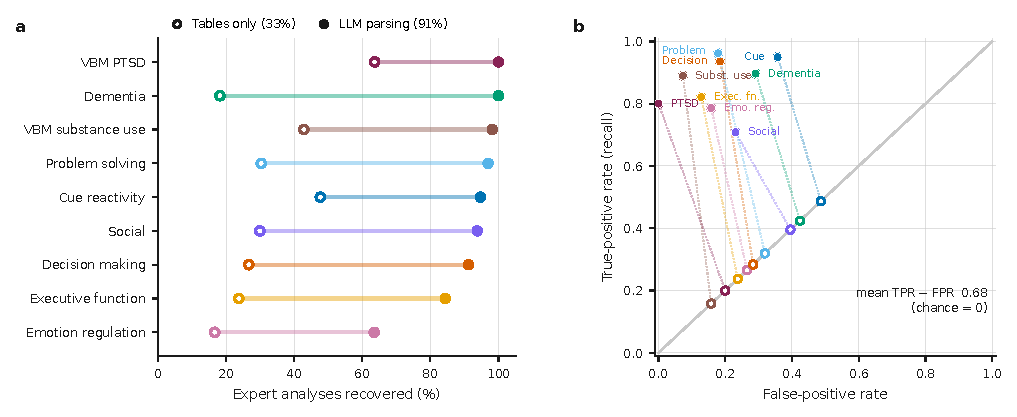
\includegraphics[width=\linewidth]{../../reports/nature_methods_figures/figure3_recover_and_select_analyses.pdf}
\caption{\textbf{LLMs extract expert curated analyses and identify relevant contrast assignments.} \textbf{a}, LLM-based parsing recovered a mean of 91.4\% of expert-curated analyses (filled markers), compared with 33.3\% when each heuristically extracted coordinate table was treated as a single analysis (open markers). Automatically extracted and expert-curated analyses were matched using optimal one-to-one assignment based on coordinate and label similarity (Methods). Articles yielding no automatically extracted analyses were excluded; post-hoc review identified the absence of coordinate data from the main text as a cause of extraction failure. \textbf{b}, True-positive rate (recall) and false-positive rate for analysis-to-contrast assignments. Filled markers represent individual projects, all of which performed above the chance diagonal (mean TPR $-$ FPR 0.68). The diagonal indicates equal true-positive and false-positive rates under random selection. Open markers show the expected performance of uniformly selecting the same number of candidate assignments as AutoNIMA, which lies on the diagonal at that project\textquotesingle s prevalence. Note that the unit is the analysis-to-contrast assignment rather than the analysis, since one analysis may be eligible for more than one contrast.}
\label{fig:parsing}
\end{figure}

We evaluated coordinate parsing and contrast assignment against expert-curated records in NeuroMetaBench. Heuristics identify candidate coordinate tables, and LLMs interpret their structure to separate coordinates into distinct analyses. Each analysis is then assessed against contrast-specific criteria using the article's full-text context.

To evaluate parsing, we matched automated analyses to expert records by coordinate and label similarity using optimal one-to-one assignment (Methods). Articles yielding no automatically extracted analyses were excluded, leaving 663 of 1,047 expert-included articles (63\%). Across projects, LLM-based parsing recovered a mean of 91.4\% of expert-curated analyses, compared with 33.3\% for heuristic table extraction alone (Fig.~\ref{fig:parsing}a), with improvements in all nine projects.

We then assessed whether the parsed analyses were assigned to the same target contrasts as expert reviewers. Across 35 annotated contrasts, pooled assignment recall was 80.9\% and precision was 53.9\% (Fig.~\ref{fig:parsing}b). These included three substance-use contrasts with expert annotations but no reference maps, which were excluded from map-level comparisons. Because the benchmark did not annotate excluded analyses, assignments involving unmatched automated analyses were counted as false positives only when all expert analyses from the corresponding article had been matched (Methods). Across projects, assignment precision was 1.8--5.6 times that expected under random selection from the same candidate pools.

\textbf{Automated synthesis improves recovery of published spatial patterns\\
}

\begin{figure}[htbp]
\centering
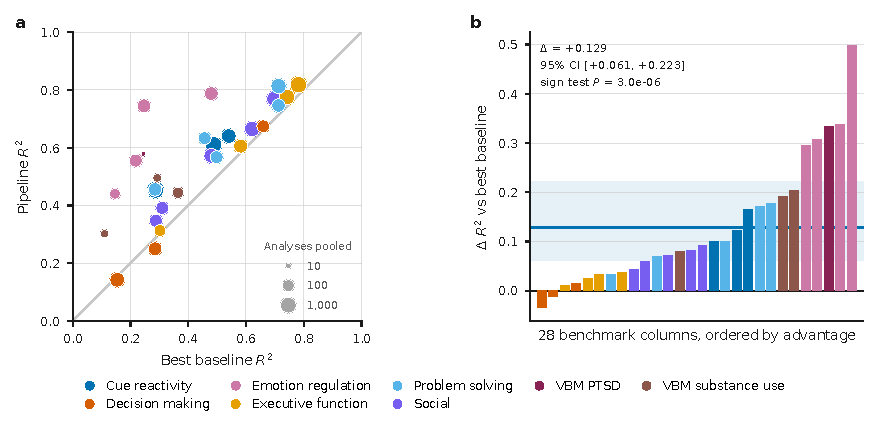
\includegraphics[width=\linewidth]{../../reports/nature_methods_figures/figure4_pipeline_vs_baseline.pdf}
\caption{\textbf{AutoNIMA improves spatial correspondence with expert-curated reference maps.} \textbf{a}, Correspondence of AutoNIMA and search-only baseline synthesis with reference maps for 28 target contrasts across eight projects, measured as squared voxelwise correlation between unthresholded maps (\emph{r}\textsuperscript{2}). Search-only baselines pooled all available analyses from PubMed searches, targeted to individual contrasts where possible, without subsequent screening or analysis selection. Points above the identity line indicate AutoNIMA maps were more similar to the reference maps than the search-only baseline. Marker area indicates the number of pooled analyses. \textbf{b}, Differences in correspondence ($\Delta$\emph{r}\textsuperscript{2}), ordered by magnitude, with the cross-contrast mean and 95\% confidence interval estimated by bootstrapping across projects (Methods). All maps were generated using multilevel kernel density analysis (MKDA). AutoNIMA achieved higher correspondence in 26 of 28 contrasts (mean r\textsuperscript{2}, 0.557 versus 0.428; mean $\Delta$r\textsuperscript{2}, +0.129).}
\label{fig:correspondence}
\end{figure}

\begin{figure}[htbp]
\centering
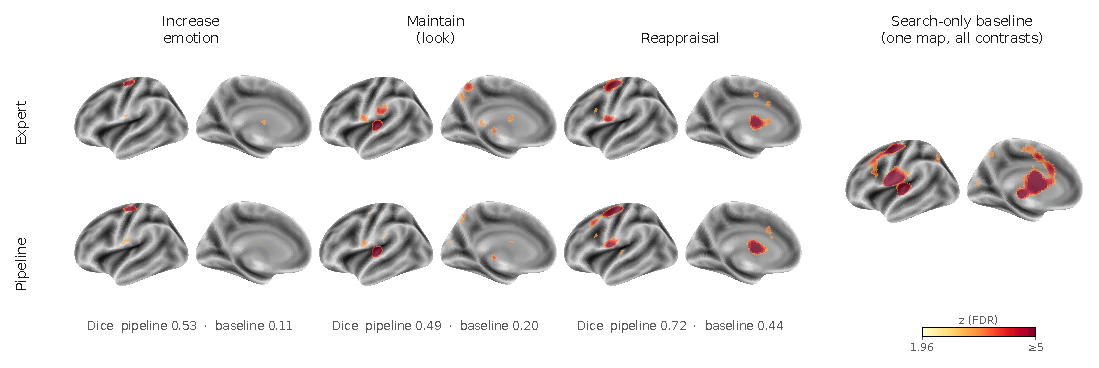
\includegraphics[width=\linewidth]{../../reports/nature_methods_figures/figure5_er_surface_contrasts.pdf}
\caption{\textbf{Analysis-level selection distinguishes emotion-regulation targets within articles.} Expert reference, search-only and AutoNIMA maps for three target contrasts: `increase', `maintain' and `reappraisal'. Maps are displayed on inflated cortical surfaces at \emph{z} \textgreater{} 1.96. A common emotion-regulation search-only baseline is shown for all three contrasts; contrast-specific searches produced similar maps. Dice coefficients quantify the spatial overlap of the expert reference and AutoNIMA maps with the search-only baseline.}
\label{fig:er-surface}
\end{figure}

We next tested whether AutoNIMA's end-to-end workflow translated improved evidence selection into more faithful recovery of published neuroimaging meta-analytic maps. To provide a robust baseline, we performed PubMed searches tailored to each target contrast in NeuroMetaBench, and pooled all resulting available analyses without subsequent article screening or analysis-level selection. Then, for both the AutoNIMA results for each project and the baselines, we performed a coordinate-based meta-analysis (CBMA) using multilevel kernel density analysis (MKDA), and computed the correspondence to NeuroMetaBench using squared voxelwise correlation between unthresholded maps (r\textsuperscript{2}; Methods). The dementia project was excluded because its reference data pooled coordinates across studies, producing analysis units that were not directly comparable with those extracted from individual articles.

Across 28 target contrasts from eight projects, AutoNIMA achieved a mean r\textsuperscript{2} of 0.557, compared with 0.428 for search-only synthesis, with higher correspondence in 26 contrasts (mean $\Delta$r\textsuperscript{2}, +0.129; sign-test P = 3.0 $\times$ 10$^{-6}$; Fig.~\ref{fig:correspondence}). Improved correspondence frequently accompanied a smaller evidence set, indicating that the benefit was not explained solely by pooling more analyses.

Improvements varied across projects, with smaller gains in decision-making and executive-function syntheses. Emotion-regulation reappraisal provided a clear example: the AutoNIMA map more closely resembled the reference spatial pattern than the search-based synthesis (Fig.~\ref{fig:er-surface}). A single reappraisal study can report separate comparisons involving increasing, decreasing or maintaining emotional responses. Article-level pooling combines coordinates across these comparisons, whereas analysis-level selection identifies those relevant to each target.

\begin{figure}[htbp]
\centering
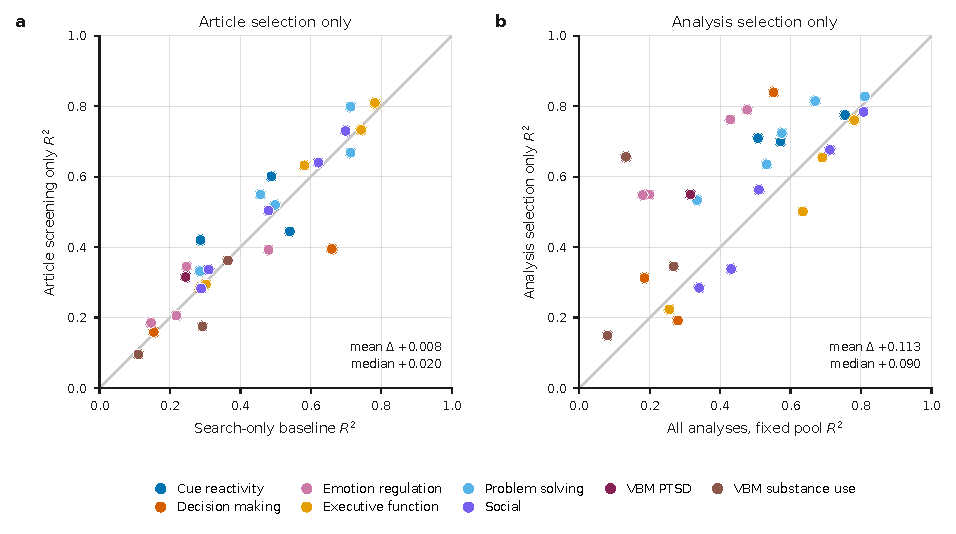
\includegraphics[width=\linewidth]{../../reports/nature_methods_figures/figure6_selection_decomposition.pdf}
\caption{\textbf{Analysis-level selection improves spatial correspondence more than article screening.} a, Correspondence of article-screening-only and search-only synthesis with reference maps for 28 target contrasts across eight projects, measured as squared voxelwise correlation between unthresholded maps (\emph{r}\textsuperscript{2}). Both conditions pooled all available analyses from their respective article sets. b, Correspondence of analysis-selection-only synthesis and its baseline with reference maps. Both conditions used the same expert-included articles from NeuroMetaBench; analysis selection retained results satisfying contrast-specific criteria, whereas the baseline pooled all parsed analyses. In both panels, points above the identity line indicate improved correspondence after screening or selection. Marker area indicates the number of pooled analyses. All maps were generated using multilevel kernel density analysis (MKDA).}
\label{fig:decomposition}
\end{figure}

\textbf{Analysis selection drives spatial correspondence}

To isolate the effects of article screening and analysis-level selection, we evaluated each component against a corresponding baseline (Fig.~\ref{fig:decomposition}). The screening-only condition applied article-level eligibility criteria and pooled all parsed analyses from retained articles; its baseline pooled all available analyses from the original PubMed search results. The analysis-selection-only condition began with expert-included articles from NeuroMetaBench and selected analyses using contrast-specific criteria, without article screening. Its baseline pooled all parsed analyses from the same expert-included articles, holding the article pool constant.

Article screening produced little additional spatial correspondence with the benchmark (mean $\Delta$\emph{r}\textsuperscript{2}, +0.008). Because 27 of 28 search baselines already targeted individual contrasts, this comparison measures the additional benefit of screening beyond targeted retrieval. In contrast, analysis selection within the expert-curated article pool improved correspondence in 19 of 28 contrasts (mean $\Delta$r\textsuperscript{2}, +0.112; median, +0.087). This mean gain was similar to that observed when adding analysis selection after article screening in the end-to-end workflow (mean $\Delta$r\textsuperscript{2}, +0.121). That end-to-end sequence also permits a direct comparison of the two steps, since both are measured against a shared baseline on the same runs and article pool: analysis selection exceeded article screening by a mean $\Delta$r\textsuperscript{2} of +0.113 (95\% CI +0.038 to +0.217, cluster bootstrap over projects; Wilcoxon signed-rank P = 0.016 across eight projects) and was the larger of the two in 20 of 28 contrasts. A separate control, applied to the same analysis-selection-only arm, showed that selected analyses outperformed equally sized random subsets in 26 of 28 contrasts (per-contrast P \textless{} 0.05, one at P = 0.0499; Fig.~\ref{fig:null}), indicating that selecting fewer analyses alone did not explain the benefit.

\section{Discussion}

LLM-guided curation can reduce the manual work of neuroimaging meta-analysis while recovering the spatial patterns reported in published syntheses. AutoNIMA integrates literature search, article screening, coordinate parsing and analysis selection within an end-to-end framework for quantitative synthesis. Evaluation against expert curation showed improved screening precision and recovery of individual analyses, culminating in greater spatial correspondence than targeted baselines in nearly all meta-analytic targets.

Our evaluation identified the recovery and selection of individual analyses as central to improved spatial correspondence with expert-curated meta-analyses. Neuroimaging articles frequently report coordinates from different populations, experimental conditions or opposing contrasts within the same table. Heterogeneous table formats make these analyses difficult to separate automatically, leading earlier frameworks to pool coordinates within articles. AutoNIMA addresses this limitation by using LLMs to interpret table structure and separate distinct analyses. Among articles yielding extracted analyses, AutoNIMA recovered 91\% of expert-curated analyses using a general-purpose LLM without fine-tuning. This demonstrates the feasibility of specialized parsing of the biomedical articles without developing a task-specific model or assembling a large labelled training dataset.

Applying contrast-specific criteria to parsed analyses improved both selection precision and spatial correspondence with expert-curated results. Article screening added little beyond targeted keyword searches, whereas selecting analyses within expert-included articles improved agreement with reference maps compared with pooling all their analyses. Emotion regulation illustrates why this distinction matters: individual articles often report comparisons involving maintaining, increasing or decreasing emotional responses\cite{Elliott2014-tu,Morawetz2025-ow}. Search-only synthesis pooled these comparisons into broader activation patterns, even with contrast-specific keyword searches. By separating and selecting the relevant analyses, AutoNIMA recovered spatial patterns that more closely resembled the expert benchmark.

The magnitude of improvement across domains nevertheless varied, with smaller gains in decision-making and executive-function syntheses. One possibility for these findings is that broad meta-analytics topics may already be represented adequately by search-based pooling, leaving less opportunity for fine-grained selection to improve the resulting maps. Alternatively, smaller gains could reflect ambiguous construct definitions\cite{Poldrack2015-pd}, imperfect criteria or limitations of LLMs to approximate domain-expert judgment. Distinguishing these explanations would require a domain expert to review the criteria and individual selection decisions---an important next step that remains difficult to scale. Nevertheless, AutoNIMA improved spatial correspondence in nearly all comparisons at modest model-use cost, suggesting substantial practical value.

However, accurate specification remains essential even when a model applied instructions consistently. In two projects, comparisons with benchmark records revealed omissions in criteria derived from published methods--- an issue that has been observed more broadly in systematic reviews\cite{Wang2020-xj}. Manually correcting these omissions improved map recovery more than subsequent LLM-assisted refinement using benchmark feedback (Fig.~\ref{fig:tiers}). These findings reinforce existing guidance that AI-assisted evidence synthesis requires human oversight, validation within the intended review context and transparent reporting of automated decisions\cite{Flemyng2025-in} For neuroimaging meta-analysis, this includes explicitly specifying participant characteristics, eligible contrasts and spatial search coverage, consistent with established methodological recommendations\cite{Muller2018-zo}. Users should check that the criteria represent the intended research question and verify their application against source articles and analyses. AutoNIMA supports this process through interactive reports documenting screening decisions and their explanations. Further community work should adapt existing guidance to automated analysis-level curation, including procedures for evaluating extraction completeness, resolving ambiguous contrasts and assessing how curation decisions affect meta-analytic maps.

The availability and fidelity of reported functional and structural neuroimaging results remain practical constraints on scalable synthesis. Only approximately one-third of NeuroMetaBench studies could be retrieved automatically from open-access sources; additional coverage depended on manual retrieval or institutional subscriptions. In addition, only 2/3rds of expert-included articles yielded extracted analyses, often because coordinates appeared only in supplementary files, which are often heterogeneous in format and difficult to parse. A more sustainable approach is to implement existing recommendations to deposit unthresholded statistical maps in repositories such as NeuroVault, accompanied by clear descriptions of the experimental contrasts \cite{Gorgolewski2015-gu,Nichols2017-sw}. Sharing effect-estimate maps and their standard errors would additionally support models that account for differences in precision across studies \cite{Salimi-Khorshidi2009-yi}. These practices would reduce reliance on extracting peak coordinates and enable image-based synthesis that retains information discarded by thresholding and peak selection, with the potential to improve sensitivity.

Shared data could also support reusable curation workflows. Neurosynth Compose already provides infrastructure for sharing expert annotations and reproducible meta-analysis specifications \cite{Kent2026-qb}. Integrating automated analysis-level curation with this infrastructure could allow researchers to inspect, refine and reuse selections across related questions. This approach aligns with proposals for living systematic reviews, which combine maintained searches with reusable, structured review data to reduce duplicated effort and incorporate new evidence\cite{Elliott2014-tu}. For neuroimaging, reusable selections could facilitate comparisons across populations, tasks and contrast directions, and enable researchers to collaborative test hypotheses in a shared environment.

In conclusion, AutoNIMA demonstrates that general-purpose LLMs can recover and select individual neuroimaging analyses to improve automated synthesis. By connecting expert-defined eligibility criteria to quantitative meta-analysis, it provides a foundation for making targeted synthesis a routine tool for investigating brain function and structure, leveraging decades of accumulated neuroimaging evidence.

\section{Methods}

\subsection{AutoNIMA Pipeline}

\subsubsection{Configuration and execution}

AutoNIMA implements an end-to-end workflow from literature search to coordinate-based neuroimaging meta-analysis. Each project is specified in a YAML configuration containing a PubMed query, article-level inclusion and exclusion criteria, retrieval sources, parsing settings and contrast-specific criteria for selecting individual analyses. Separate screening configurations allow broader criteria to be applied to abstracts and more detailed criteria to full texts. The Python pipeline executes the workflow sequentially, recording progress and outputs in a dedicated project directory. AutoNIMA caches interim outputs, enabling resumption of workflows and minimizing unneeded computation external API calls.

The four LLM-assisted stages---abstract screening, full-text screening, coordinate parsing and analysis selection---access models through the OpenAI Python library. Model identifiers and API endpoints are configurable, allowing use of OpenAI-compatible providers. For this evaluation, all four stages used the general-purpose model gpt-5-mini-2025-08-07. Each stage used a task-specific prompt template combining general instructions with relevant user-defined configuration values, including project-specific eligibility criteria. Output formats were defined using Pydantic schemas compiled to JSON Schema, and model responses were validated against these specifications. Stage-specific outputs included parsed analyses and coordinates, eligibility decisions, criterion-level assessments and supporting explanations.

\subsubsection{Literature search}

Candidate articles were identified through PubMed using the Entrez API and project-specific queries. Search queries, date restrictions and search dates were recorded in the project configurations and run records. Because the present evaluation focused on automated curation rather than search performance, we transcribed the published PubMed queries verbatim and refined them through expert review and LLM assistance to improve retrieval of benchmark included articles.

\subsubsection{Article screening}

The screening workflow proceeded from abstract screening to full-text retrieval and screening. Abstract screening provided a lower-cost initial filter for clearly ineligible articles, whereas full-text screening was performed using the more complete information available in the retrieved article. The same general screening procedure was used at both stages, with the information supplied to the model differing according to the stage. Project-specific screening criteria were specified in the pipeline configuration and incorporated into the screening prompts. In configurations used in this evaluation, abstract-screening criteria were intentionally more permissive to account for the incomplete information available in abstracts, whereas full-text screening used the complete set of project-specific inclusion and exclusion criteria.

At each screening stage, the model was instructed to evaluate the supplied article information against the configured criteria. For each inclusion criterion, the model reported whether the criterion was satisfied, and for each exclusion criterion, whether the criterion was triggered. The model was instructed to exclude an article if any required inclusion criterion was not satisfied or if at least one exclusion criterion was triggered. In addition to these criterion-level assessments, the model returned a Boolean eligibility decision and free-text reasoning explaining the decision. The Boolean decision determined whether the article proceeded to subsequent stages of the pipeline. Thus, articles were retained when all applicable inclusion criteria were satisfied and no exclusion criterion was triggered.

\textbf{Full text retrieval}

Full texts for articles that passed abstract screening were retrieved using sources specified in the project configuration. Supported sources include PubMed Central (PMC), publisher APIs, and user-provided article files. PubMed Central articles were retrieved using \emph{pubget}, an open-source Python library for querying and fetching texts from PMC. Publisher retrieval is supported through text-mining APIs, including the Elsevier Full Text API and Springer Nature APIs; access to these services requires API registration using the applicable institutional or text-and-data-mining access rights. User-provided full-text HTML can also be supplied directly, including article HTML files obtained through institutional access. For the present evaluation, we supplemented automated retrieval with manually downloaded article files obtained using institutional access where possible. We were unable to include articles only available as PDF files, or for which access could not be obtained.

Importantly, AutoNIMA distinguishes retrieval failures from eligibility decisions. Records for which no usable full text could be obtained are marked as \emph{unavailable}, whereas articles for which the available text was incomplete were identified as \emph{incomplete} by the LLM screener as part of the screening instructions. Neither condition was treated as an LLM screening error in the evaluation, because the failure concerned availability or quality of the retrieved article text rather than the model\textquotesingle s eligibility judgment.

\subsubsection{Coordinate parsing into analyses}

For articles retained after full-text screening, candidate coordinate tables were identified and extracted for further processing using deterministic heuristics. An LLM was then provided with each table, together with its caption and footnotes, and instructed to extract valid stereotactic coordinates and group them into the distinct statistical analyses represented in the table. The parsing prompt used a two-pass procedure: first identifying analysis-defining axes and result blocks, and then assigning each coordinate to the appropriate combination of these axes. Analysis boundaries were defined by explicit changes in contrast or comparison, contrast direction, activation or deactivation, participant group, treatment, task condition, session, time point, parametric effect, or other explicitly labeled analysis dimensions. The parser also handled analysis structure encoded in multi-level or repeated column headers, allowing a single table row to contribute coordinates to multiple analyses when the table reported multiple independent analysis blocks.

The parser was instructed not to treat descriptive anatomical subdivisions as separate statistical analyses unless the source explicitly identified them as distinct statistical maps. Similarly, separate whole-brain and region-of-interest result blocks were treated as distinct analyses when explicitly labeled. When no explicit analysis-defining distinction was present, the table was treated as a single analysis. The parser extracted coordinates only from explicitly identified spatial coordinate fields, required complete three-dimensional coordinate triples, and recorded the reported coordinate space when explicitly identified as MNI or Talairach. Where available, same-row statistical values were also retained with their reported statistic type.

\subsubsection{Analysis-level selection}

Parsed analyses were subsequently evaluated against the project-specific, contrast-specific inclusion and exclusion criteria using the full text of the corresponding article. This evaluation was performed on an article-by-article basis: for each article, the LLM was provided with the full-text article together with all parsed analyses from that article and the complete set of target-contrast criteria. For each parsed analysis and each target contrast, the model evaluated whether the analysis satisfied the corresponding inclusion and exclusion criteria, producing a Boolean assignment for every analysis--target contrast pair. These decisions were represented as an analysis $\times$ target-contrast Boolean inclusion matrix.

The criteria could include global criteria applicable to all target contrasts as well as target-specific criteria. Global criteria were applied first as a hard gate: an analysis was excluded from a target contrast if a required global inclusion criterion was not satisfied or if a global exclusion criterion applied. Analyses passing the global criteria were then evaluated against the local inclusion and exclusion criteria for each target contrast. An analysis was assigned to a target contrast when all required criteria were satisfied and no applicable exclusion criterion was triggered. Because each analysis--target contrast pair was evaluated independently, a single analysis could be assigned to multiple target contrasts when it satisfied the criteria for each. As with article-level screening, the model provided criterion-level assessments and a free-text rationale for each decision.

\subsubsection{Meta-analytic modeling}

Coordinates from analyses selected for each target contrast were submitted to coordinate-based meta-analysis independently for each target. Selected analyses and their coordinates were represented in the NeuroImaging Meta-Analysis Data Structure (NiMADS), a standardized format for representing neuroimaging studies, analyses, and reported coordinates, enabling interoperability with the NiMARE library for neuroimaging quantitative meta-analysis. For each target contrast, the resulting coordinate set was used to generate a spatial meta-analytic map using the corresponding coordinate-based meta-analysis procedure specified for the reference analysis. \cite{Salo2023-fb}

NiMARE exposes a wide range of meta-analytic algorithms (KDA, MKDA, ALE) and multiple correction methods (FWE, FDR), which can be specified by users run time through the AutoNIMA interface. For this evaluation all analyses were executed using MKDA using NiMARE's default configuration. Each coordinate was convolved with a sphere of 10 mm radius; where spheres overlapped, the maximum was retained; the resulting study-wise modelled activation maps were combined into an MKDA density statistic; and those summary statistics were converted to \emph{p}-values against an approximate null distribution rather than by Monte Carlo resampling. Multiple comparisons were controlled by the Benjamini--Hochberg false discovery rate (FDR) procedure at \emph{q} = 0.05 under the independence assumption. Maps were estimated using the MNI152 template, and a focus-counter diagnostic was run for each fit. For each meta-analytic target, NiMARE produced an unthresholded \emph{z} map with its statistic and \emph{p} maps and the FDR-corrected \emph{z} and \emph{p} maps and a cluster table; the two similarity metrics read the unthresholded and the corrected map respectively.

\section{Benchmark and Evaluation Procedure}

We evaluated AutoNIMA using NeuroMetaBench, a companion benchmark of nine published, expert-conducted neuroimaging meta-analyses. For each project, the benchmark provides article inclusion records and curated data identifying the analyses, coordinates and target-contrast assignments used in the reference synthesis. These records support evaluation of article screening, recovery of individual analyses, assignment of analyses to target contrasts and spatial correspondence of the resulting maps. Benchmark construction is described in the companion report.

The benchmark configurations contained 35 annotated targets across 9 projects of diverse topics. Three targets from the VBM of Substance Abuse project---cannabis, opioids and stimulants---were excluded from the reported target set because the source review reported no significant clusters for these targets, leaving 32 total targets. The primary map comparisons additionally excluded the four dementia targets, leaving 28 contrasts across eight projects. The dementia reference records pooled coordinates across contributing studies, preventing consistent attribution to individual articles and comparison with article-level automated extraction. Dementia was retained in article-screening and parsing evaluations and in the exploratory criteria-refinement analysis.

\subsubsection{Article-screening}

Article-level precision was defined as the proportion of retained articles present in the benchmark inclusion list. At the final analysis-selection stage, an article was considered retained if at least one of its analyses was selected for a target contrast.

Recall was adjusted for availability to distinguish screening decisions from failures of retrieval or extraction. The search-stage denominator comprised benchmark articles returned by the PubMed search, making recall at this stage 100\% by construction. The same denominator was used for abstract screening. At full-text screening, benchmark articles lacking usable full text were removed from the denominator. At analysis selection, benchmark articles that reached coordinate extraction but yielded no parsed analyses were additionally removed. By removing articles with no usable inputs for each stage, the recall metrics specifically measure the performance of the LLM model at each stage of selection.

To examine the influence of the candidate article pool on measured screening performance, we repeated screening with the same eligibility criteria using candidate lists available from the original reviews in three projects that made that list available: dementia, emotion regulation and social cognition. We compared these results with screening of the articles returned by AutoNIMA\textquotesingle s PubMed searches. The emotion-regulation list covered only part of the literature considered in the original review, limiting its use as a complete reconstruction of the original screening pool.

\subsubsection{Recovery of expert-curated analyses from table parsing}

Automatically parsed analyses were matched to expert-curated records within the corresponding article using optimal one-to-one assignment with the Hungarian algorithm over pairwise similarities. Hungarian matching prevented a single automated analysis from matching multiple expert records, and attempted to match the two best matching automated-manual pairs. This was necessary in part because the expert benchmark only annotated included analyses--- that is, analyses that were not relevant to any of the target contrasts were never entered by annotators.

\textbf{Pairwise similarity.} Each candidate pair receives a combined score \emph{s} = 0.70 $\cdot$ $s_{\mathrm{coord}}$ + 0.30 $\cdot$ $s_{\mathrm{label}}$. A greater weight was given to Coordinates, as they are the most objective evidence of matching, whereas labels were annotator assigned and not necessarily verbatim from article prose.

\begin{itemize}
\item
  \textbf{$s_{\mathrm{coord}}$, coordinate agreement.} Expert and automated coordinates are first paired by a second Hungarian assignment, this one minimising Euclidean distance in millimetres, which makes the score independent of the order coordinates appear in. Each paired distance \emph{d} is mapped to a similarity by a piecewise-linear curve: 1.0 for \emph{d} $\leq$ 1 mm, 0.9 for \emph{d} $\leq$ 2 mm, then falling linearly to 0.6 at 4 mm, 0.2 at 8 mm and 0 at 12 mm and beyond. The mean of the paired similarities is multiplied by a coverage penalty, min($n_{\mathrm{expert}}$, $n_{\mathrm{auto}}$) / max($n_{\mathrm{expert}}$, $n_{\mathrm{auto}}$), so an automated analysis that recovers the right peaks but the wrong number of them is discounted in proportion. A bonus of 0.05 is added when the two coordinate sets are identical to one decimal place, and the result is clipped to {[}0, 1{]}.
\item
  \textbf{$s_{\mathrm{label}}$, analysis-name agreement.} The maximum ratio over four comparisons of the expert and automated analysis names --- full against full, base against base, and each against the other\textquotesingle s base --- where the base is the text before the first semicolon and both strings are case-folded and whitespace-normalised. Taking the maximum lets a fully-qualified label match a truncated one without penalty.
\end{itemize}

\textbf{Acceptance.} A pair counts as a recovered analysis at \emph{s} $\geq$ 0.55. However, a coordinate-driven override additionally accepts a pair whose combined score is low but whose geometry is unambiguous, when any of the following holds: $s_{\mathrm{coord}}$ $\geq$ 0.90; $s_{\mathrm{coord}}$ $\geq$ 0.80 with the two coordinate sets of equal size and at least three coordinates; or equal-sized sets of at least three coordinates with $\geq$ 90\% of pairs within 8 mm and a median paired distance $\leq$ 6 mm. The override exists because an automated analysis can reproduce an expert analysis exactly and still score poorly on the label, having inherited a table caption rather than a contrast name. Match at high confidence is defined as s$\geq$0.75, or a coordinate match as described below.

\textbf{Coordinate space during matching.} Coordinates in NeuroMetaBench were frequently converted to MNI space even if the original coordinates were reported as Talairach. To enable automated matching, we detected converted records based on if they reported decimal precision, and transformed the annotated coordinates back to Talairach space using NiMARE's built in transformer. However, to ensure our assumption was correct, we scored the similarity of three variants of each such record --- the coordinates as published, and both the Talairach-to-MNI and MNI-to-Talairach re-expressions --- and kept the best-scoring one. The two converted variants are allowed to qualify as an exact set under an axis-wise tolerance of $\pm$ 1.0 mm, which the as-published variant is not. This transform is applied only for matching; it is independent of the space handling inside the meta-analysis (see \emph{Meta-analytic modeling}).

\subsubsection{Analysis-level selection}

To evaluate LLM performance in matching analyses to target contrasts, we computed precision and recall of analysis-to-contrast assignments relative to the expert benchmark, separately for each target contrast. Selection performance was evaluated at the level of analysis-to-contrast assignments because a single analysis could satisfy the criteria for multiple target contrasts.

\textbf{Exhaustive matching strategy.} The expert benchmark annotated only analyses that were included in the reference meta-analysis; analyses that were excluded were not annotated, and their coordinates were therefore not available for comparison. Scoring only automated assignments that matched an expert annotation would consequently bias precision upward: although models could correctly match included analyses to the appropriate target, they could also assign analyses that should have been excluded altogether. To conservatively account for these assignments, we used an exhaustive matching strategy. LLM assignments that did not match an expert annotation were counted as false positives only after all expert-annotated analyses from the corresponding article had been matched with high confidence to automated analyses. Because the benchmark did not annotate analyses that were present in an article but excluded from the reference meta-analysis, an unmatched automated analysis could not otherwise be assumed to represent a false-positive selection. Once all expert-annotated analyses had been matched, every remaining automated analysis entered the scoring universe for that contrast: those the pipeline had assigned to the contrast were counted as false positives, and those it had not were counted as true negatives.

Of the 11,126 analysis-to-contrast assignments in the scoring universe, 5,805 (52.2\%) were automated assignments with no matching expert annotation. Of these, 1,399 had been matched by an LLM to a target contrast and were counted as false positives; the remaining 4,406 were not selected and were counted as true negatives. Applying this strategy reduced pooled precision from 0.863 to 0.539 while leaving recall unchanged at 0.810.

\textbf{Metrics.} For each target contrast, precision, recall, and the corresponding ROC quantities were computed as

\begin{equation*}
\begin{aligned}
\mathrm{Precision} &= \frac{TP}{TP + FP}, &
\mathrm{Recall} = \mathrm{TPR} &= \frac{TP}{TP + FN}, &
\mathrm{FPR} &= \frac{FP}{FP + TN},
\end{aligned}
\end{equation*}

where $TP$, $FP$, $FN$ and $TN$ denote true-positive, false-positive, false-negative, and true-negative analysis-to-contrast assignments, respectively. Pooled estimates were calculated by summing true positives, false positives, false negatives, and true negatives across projects before computing the corresponding metrics. Project-level receiver operating characteristic (ROC) displays plotted $\mathrm{TPR}$ against $\mathrm{FPR}$.

\textbf{Random-selection comparisons.} Random-selection baselines were generated from the candidate assignment pool for each project. For a fully labeled pool of (N) assignments, uniformly selecting (k) assignments yields an expected true-positive rate and false-positive rate of (k/N), with expected precision equal to the prevalence of expert-positive assignments in the scoring universe. Precision enrichment was calculated relative to this prevalence. Random reference points were calculated analytically rather than by Monte Carlo sampling.

\subsubsection{Coordinate-based meta-analysis and spatial correspondence}

Meta-analytic maps were generated as described above (\emph{Meta-analytic modeling}). The same estimation procedure and settings were used for the automated, baseline, and reference arms.

\textbf{Spatial correspondence strategy.} For each automated meta-analysis, spatial correspondence was evaluated by comparing its resulting statistical map with a reference map reconstructed from the expert-curated coordinate records. Reference maps were reconstructed using the same MKDA procedure, irrespective of the method used in the original publication (e.g., ALE). The comparisons therefore assess correspondence with reconstructions from published curation records rather than exact reproduction of the statistical analyses reported in the source publications.

Correspondence was also evaluated relative to a search-only baseline. The baseline included every analysis parsed from every article returned by the literature search for the target, without LLM screening or analysis-level selection, and applied the identical meta-analytic procedure. For contrasts with a dedicated search, that targeted search defined the baseline; for contrasts that were not separable search topics, such as effect direction within a single paradigm, the project\textquotesingle s broad search was used.

The effect of automated selection was expressed as the difference in correspondence between the automated and baseline arms:

\begin{equation*}
\Delta M = M_{\mathrm{automated}} - M_{\mathrm{baseline}},
\end{equation*}

where $M$ denotes the spatial correspondence metric.

\textbf{Spatial correspondence metrics.} The primary measure was the squared Pearson correlation (r2r\^{}2) between unthresholded statistical maps over the full image volume, without applying a brain mask.

\begin{equation*}
r = \frac{\sum_{v=1}^{V}(X_v-\bar X)(Y_v-\bar Y)}{\sqrt{\sum_{v=1}^{V}(X_v-\bar X)^2}\,\sqrt{\sum_{v=1}^{V}(Y_v-\bar Y)^2}},\qquad M=r^2.
\end{equation*}

Dice overlap was used as a secondary measure for thresholded maps and illustrative map comparisons. Maps were thresholded at $z > 1.96$ using the FDR-adjusted $z$-images, and Dice overlap was calculated as

\begin{equation*}
\mathrm{Dice}(A,B) = \frac{2|A\cap B|}{|A|+|B|},
\end{equation*}

where $A$ and $B$ denote the sets of suprathreshold voxels. Differences between the automated and baseline arms were calculated as

\begin{equation*}
\Delta\mathrm{Dice} = \mathrm{Dice}_{\mathrm{automated}} - \mathrm{Dice}_{\mathrm{baseline}}.
\end{equation*}

\subsubsection{Random-subset comparison}

For each target in the map-level random-selection control, we drew 500 random subsets from the candidate analysis pool used for the observed selection. Each subset contained the same number of distinct analyses as the selected set. MKDA was repeated for each subset using the same settings and reference map as the observed comparison. This procedure held the number of pooled analyses constant while varying their identities.

Observed r\textsuperscript{2} was compared with the mean and 5th--95th percentile range of the random-subset distribution. The one-sided empirical P value was calculated as (b + 1)/501, where b was the number of random subsets with correspondence at least as high as the observed result. The reported per-contrast threshold of P \textless{} 0.05 was not adjusted across contrasts. Percentile ranges describe variation among random subsets, not confidence intervals for the observed estimate. {[}Confirm which pipeline arm supplies this control\textquotesingle s candidate pool and selected set; author check 10.{]}

\subsubsection{Criteria refinement and benchmark feedback}

Initial project criteria were drafted to follow the eligibility descriptions in the source publications. Configurations were registered as initial transcriptions (verbatim), manually revised configurations (manual), the configurations selected for the principal evaluation (best). The registry retained configuration versions, associated runs and reasons for selecting the principal configurations.

Manual review identified substantial mis-specification in two initial specifications. Further revisions used LLM assistance and benchmark feedback. Both forms of revision were informed by benchmark comparisons, and the principal results used the selected best configurations. These evaluations therefore did not constitute an independent held-out test of criteria refinement as, revising prompts or eligibility criteria using benchmark performance can introduce optimism into the reported estimates.

The exploratory progression analysis compared within-project mean r\textsuperscript{2} between distinct evaluated configurations. The initial-to-manual comparison involved dementia and cue reactivity; the manual-to-best comparison involved cue reactivity and social cognition..

\subsubsection{Statistical inference and uncertainty estimation}

Two analyses were performed: evaluation of the end-to-end change in map correspondence relative to the baseline, and decomposition of this change into article-selection and analysis-selection components. The project was treated as the independent unit of inference rather than the contrast. Contrasts within a project share the same article pool, screening run, and reference record and are therefore not independent observations. Resampling at the contrast level would consequently underestimate uncertainty.

\textbf{Pipeline versus baseline.} End-to-end change in map correspondence ($\Delta$\emph{r}\textsuperscript{2}) was summarized across 28 evaluated contrasts from eight projects. The 95\% confidence interval for the mean change was estimated using a project-level percentile bootstrap with 20,000 resamples (random seed = 0). Projects were sampled with replacement, retaining all contrasts within each selected project, and the mean contrast-level change was calculated for each resample.

The proportion of contrasts showing a positive change was additionally evaluated using a two-sided exact binomial test against a null probability of 0.5. Ties were counted as non-positive changes rather than excluded. No ties occurred for \emph{r}\textsuperscript{2}; for the Dice robustness analysis, four contrasts had a score of 0.000 for all arms and were therefore counted as non-wins. Because the binomial test treats contrasts as independent observations, its \emph{P} value was considered nominal and was reported as a complementary analysis to the project-level bootstrap confidence interval.

\textbf{Decomposition of the margin.} The baseline, screening-only, and full-pipeline arms were derived from the same article pool, such that the article-selection and analysis-selection components were additive and summed to the end-to-end change for each contrast. The difference between these two components was therefore evaluated as a paired comparison. The primary confidence interval was obtained using the same project-level cluster bootstrap described above. As complementary analyses, the difference was evaluated using a Wilcoxon signed-rank test and paired \emph{t}-test across the eight project-level means, and a sign test across contrasts.

The annotation-only arm shown in Fig.~\ref{fig:decomposition}b was initialized from the expert inclusion list and therefore used a different article pool. Its gain was consequently reported descriptively and was not included in the decomposition or formally compared with the other arms, because these conditions do not constitute paired observations from the same article pool.

\subsubsection{Model-use costs}

Model-use costs were estimated from recorded input, cached-input, and output token consumption using per-stage token accounting. Abstract screening and full-text screening usage were measured over 708 and 1,211 model calls, respectively, across two projects each; coordinate parsing and analysis selection were measured over 1,299 and 1,091 calls, respectively, across three projects each. Token counts were converted to US dollar costs using the gpt-5-mini-2025-08-07 rates applicable at the time of measurement (4 September 2026):US\$0.25 per million input tokens and US\$2.00 per million output tokens.

\subsubsection{Data availability}

Project configurations, evaluation tables, analysis assignments and generated maps supporting the results are available at \url{https://github.com/neurostuff/autonima-results/}. Third-party texts are not included in the repository due to copyright restrictions, but PubMedCentral articles can be readily redownloaded using pubget.

\subsubsection{Code availability}

AutoNIMA is available under the MIT License at \url{https://github.com/neurostuff/autonima}. The version used in this study was v0.0.1. Scripts for reproducing the evaluations and figures, together with the computational environment specification, are available at \url{https://github.com/neurostuff/autonima-results/}. Code used to construct the benchmark is available at \url{https://github.com/neurostuff/neurometabench/}.

\subsubsection{Use of generative AI}

The use of LLMs for screening, coordinate parsing and analysis selection constituted the method evaluated in this study and is described above. Separately, the authors used OpenAI Codex and Anthropic Claude to assist with software development of the main AutoNIMA package. During the preparation of this manuscript, the authors utilized OpenAI GPT-6 Astra to assist with editing and revising text for clarity, readability, and flow. In all instances, the AI-generated text was critically reviewed, edited, and revised by the authors to ensure accuracy and originality. The authors take full responsibility for all content presented in this manuscript, including any portions assisted by AI.

\subsubsection{}

\subsubsection{}
